\chapter[Resilient State Estimation and Cyber-Attack Reconstruction]{Resilient State Estimation and Cyber-Attack Reconstruction for Connected Autonomous Vehicles}\label{chp2_chap}
\chaptermark{Resilient State Estimation and Cyber-Attack Reconstruction}

\objectif{The primary objective of this work is to develop a resilient controller and state observers capable of:

Estimating unmeasured quantities necessary for the SA-ACC.

Detecting and reconstructing false data injected into the communication channel exactly and in finite time.

Compensating for these attack signals to maintain vehicle autonomy.}

%%%%%%%%%%%%%%%%%%%%%%%%%%%%%%%%%%%%%%%%%%%%%%%%%%%%%%%%%%%%%%%%%%%%%%%%%%%%%%%%%%%%%%%%%%%%%%%%%
\section{Introduction and Problem Statement}
%%%%%%%%%%%%%%%%%%%%%%%%%%%%%%%%%%%%%%%%%%%%%%%%%%%%%%%%%%%%%%%%%%%%%%%%%%%%%%%%%%%%%%%%%%%%%%%%%

\subsection{Context}
The advent of autonomous and connected vehicles (CAVs) represents the future of mobility, leveraging advanced technologies such as artificial intelligence to ensure automated driving. These systems promise increased safety, improved energy efficiency, and a comfortable driving experience by utilizing Vehicle-to-Vehicle (V2V) and Vehicle-to-Infrastructure (V2I) communication. However, the reliability and availability of sensors constitute critical challenges that hinder the full development of these vehicles.



\subsection{The Cyber-Security Challenge}

A specific vulnerability in CAVs is the susceptibility of the communication channels to cyber-attacks. The VEHALSECU project specifically addresses the problem of estimating necessary variables for a Semi-Autonomous Adaptive Cruise Control (SA-ACC) system when communication is corrupted by cyber-attacks. Specifically, False Data Injection (FDI) attacks can bypass conventional security measures, allowing attackers to compromise sensor measurements and disrupt network operations.


While machine learning techniques have been proposed for detection, they are often computationally expensive and unsuitable for the real-time constraints of embedded vehicle control. Furthermore, existing research often assumes attack signals are constant, which limits the scope of protection against time-varying or arbitrary unbounded attacks.

% \begin{figure}[H]\centering
% \includegraphics[width=.5\linewidth]{ch2/fig/Saturation_voxel_size.png}
% \caption{Une description avec la légende associée et sa référence.}
% \label{fig2_example}
% \end{figure}

\section{Design of Resilient Observers}
The core scientific challenge lies in the "Unknown Input Observer" (UIO) design. Standard UIOs require two mathematical conditions: strong detectability and a specific rank condition on the system matrices18181818. While the SA-ACC model satisfies the detectability condition 19, it fails the rank condition ($rank(CW) \neq rank(W)$)20. Consequently, standard UIOs cannot be directly applied.To overcome this, two distinct methodological approaches were developed: a discrete-time approach using delayed observations and a continuous-time approach using sliding mode differentiation.

\subsection{CACC modeling subject to cyberattack}
%----
Basically, the dynamics of $i^{th}$ vehicle are a Position-Velocity-Acceleration third-order linear model given by the following set of equations:
\begin{equation}\label{eq_1}
      \left\{ \begin{array}{l}
        \dot{p}_i(t) =v_i(t) \\
        \dot{v}_i(t)  =a_i(t) \\
        \dot{a}_i(t)  =\frac{1}{\tau_i} u_i(t)-\frac{1}{\tau_i} a_i(t)\end{array}\right.
\end{equation}  
where
\begin{itemize}
\item $p_i(t), v_i(t)$ and $a_i(t)$ denote the position, velocity and
acceleration of the $i^{th}$  vehicle, respectively;
\item $u_i(t)$ is the $i^{th}$ vehicle control input representing the desired
driving/braking force or acceleration;
 \item $\tau$ is the engine's constant time lag. 
 \end{itemize}
 %
%For the sake of brevity and simplification, the system~\eqref{eq_1} can be written under the following condensed matrix form:
%\begin{equation}
%\dot{x}_{i}(t) = 
%\left[\begin{array}{c c c}{{0}}&{{1}}&{{0}}\\
%{{0}}&{{0}}&{{1}}\\ 
%{{0}}&{{0}}&{{-\tau^{-1}}}\end{array}\right]x_{i}(t)
%+\left[\begin{array}{c}{{0}}\\ {{0}}\\ 
%{{\tau^{-1}}}
%\end{array}\right]u_{i}(t)
%\end{equation}
%where $x_i(t) \triangleq \begin{bmatrix} p_i(t) & v_i(t) & a_i(t) \end{bmatrix}^{\top}$.
%
% The output yi of vehicle i is given by\\
%
% $y_{i}(t)=C x_{i}(t)=\left[{\begin{array}{r r r}{1}&{0}&{0}\\ {0}&{1}&{0}\end{array}}\right]x_{i}(t).$
% In this study, the control strategy is similar to the one that
% is presented [bla] 
% were x = [x1, v1, a1] > R2n are the states of all the vehicles in the platoon, A 2 R2n ⇥ 2n, B 2
% R2n⇥2, C 2 R2n⇥2n,
%
% The desired spacing between vehicles in the constant time-gap spacing policy is not constant but is linear function of speed:
% \begin{equation}
%     Desired\;Spacing=L+h\dot{x}_{i}
% \end{equation}
%

%{\color{red}
The actual spacing between vehicles are $\varepsilon_{i,act} = p_{i-1} - p_{i}$ 
%\begin{equation}
%    \varepsilon_{i} = p_{i-1} - p_{i}
%\end{equation}
and the desired spacing between 
vehicles in the constant time-gap spacing policy is given by $\varepsilon_{i,des} = {L} + h{v}_{i}$.
%\begin{equation}
 %   \varepsilon_{i,des} = {L} + h{v}_{i}.
%\end{equation}
%}
It follows that the spacing error can be written as: 
\begin{equation} \label{spacing_e}
    \varepsilon_{i,des} -\varepsilon_{i,act} \triangleq p_{i}-p_{i-1}+L+h{v}_{i} = \varepsilon_{i} + h{v}_{i},
\end{equation}
where ${L}$ is the minimum safety distance and $h$ is the time-gap.
Then, the controller $u_{\text{i}}$ is given by~\cite{rajamani2002semi}:

\begin{multline}\label{controller}
        u_{\text{i}} = -k_{1}{a}_{i-1}+(k_{1}+h k_{1}k_{2}){a}_{i}\\
        -\frac{1}{h}(1-h k_{1}k_{2})\dot{\varepsilon}_{i} -\frac{k_{2}}{h}\varepsilon_{i}-k_{2} {v}_{i}
\end{multline}
where ${a}_{i-1}$ is the acceleration of the preceding vehicle obtained by using inter-vehicle communication.
The scalar gains $k_1$ and $k_2$ are the controller design parameters to be designed according to the detailed procedure introduced in~\cite{rajamani2002semi}. 
%It has been shown in~\cite{rajamani2002semi} that if the gain $k_1$ is chosen such as to satisfy the constraint $-k_{1}h >\tau$, then the CACC controller \eqref{controller} is string stable, independently from the value of $h$. 

The controller $u_{\text{i}}$ defined in~\eqref{controller} is convenient in perfect situation where the acceleration of the preceding vehicle, $a_{i-1}$, provided through V2V communication channel is not corrupted by intruders. Unfortunately, in CACC platoons, the V2V communication may provide unreliable acceleration due to potential tampering by attackers. %Hence the interest to develop a judicious resilient controller taking into account the presence of injected false data in the communication channel.% or any other cyberattack scheme. 
%
% The next section is devoted to this issue by mathematically modeling the CACC system subject to cyberattack. We consider the more general case where disturbances affect the dynamics and the measurements of the model, which leads to a robust and resilient CACC controller.
%
%================
%\subsection{CACC model representation subject to cyberattack}
%--
%As emphasized in the previous section, the CACC controller~\eqref{controller} is convenient and reliable if it is not subject to cyberattacks and/or any other internal or external disturbances. 
To develop a resilient controller to cyberattacks, we have to consider the attack signal in the design of the controller. To this purpose, we assume that the following vehicle receives the signal $\mu(t)$  corrupted by injected false data in the wireless communication channel:
\begin{equation}\label{ali_e1}
\mu(t) = a_{i-1}(t) + f^c(t)
\end{equation}
where $a_{i-1}(t)$ is the true acceleration and $f^c(t)$ is the additive cyberattack signal. This cyberattack scheme under additive false signals can cover several cyberattack architectures. These may include message falsification attacks, spoofing attacks, and denial of service~(DoS) attacks. For instance, in the DoS case, by using the differential mean value theorem, there exists $\theta_t \in [t-\tau(t),~ t]$ such that the delayed signal $a_{i-1}(t-\tau(t))$ can be represented as follows:
\begin{align}\label{ali_e2}
 \mu(t) = a_{i-1}(t-\tau(t)) &= a_{i-1}(t) \underbrace{- \frac{{\rm d}a_{i-1}}{{\rm d}t}(\theta_t) \tau(t)}_{f^c} \notag \\
 &= a_{i-1}(t) + f^c.
\end{align}



%\bigskip
%%
%The transmitted signal $\mu = a_{i-1}(t) + f^c $ can be represented while considering cyberattacks.
%%\begin{remark}
%%{\color{red}{je ne comprend pas la phrase ???????}
%Several common types of attacks involve adding false signals to a transmission. These include message falsification attacks, replay attacks, and denial of service (DOS) attacks. For instance, with a DOS attack, it is possible to express the delayed signal $a_{i-1}(t-\tau_d)$ using Taylor's series expansion.
%\begin{equation}\mu(t-\tau_d ) = a_{i-1}(t) -\dot{a}_{i-1}(t)\tau+ \textit{H.O.T}
%\end{equation}
%So the delay can simply be presented as :
%\begin{equation}
%\mu(t-\tau_d ) = a_{i-1}(t) + f_d. 
%\end{equation}
%% About why send acceleration rather than send control input $u$, from many papers. Maybe acceleration is more versatile, because, in case of a non-homogenous platoon, the control input is not the same. 
%%}
%%\end{remark}

Under a cyberattack, the following vehicle receives $\mu$ and will utilize it in its controller. Then, instead of~\eqref{controller}, the controller $u_{\text{i}}$ will be implemented as follows:
\begin{align}\label{control_uc}
        u_{\text{i}}&=-k_{1} \mu(t) + (k_{1}+h k_{1}k_{2}){a}_{i} \notag\\
        &\quad-\frac{1}{h}(1-h k_{1}k_{2})\dot{\varepsilon}_{i} -\frac{k_{2}}{h}\varepsilon_{i}-k_{2} {v}_{i}.
\end{align}
%
%% \begin{align} \label{control_uc}
%%         u_{s y n}&=\left(h k_1 k_2\right) \mu-\left(k_1+h k_1 k_2\right) f^c-k_2 \dot{x}_i  \notag\\
%%        & +\frac{k_2}{h} \delta_i-\left(k_1+h k_1 k_2\right) \ddot{\delta}_i\notag\\
%%        &+\frac{1}{h}\left(1-h k_1 k_2\right) \dot{\delta}_i -\frac{k_2}{h}\left(L-l_{i-1}\right)
%%     \end{align}
%\begin{align}\label{control_uc}
%        u_{\text{i}}&=-k_{1}\mu+(k_{1}+h k_{1}k_{2}){a}_{i}-\frac{1}{h}(1-h k_{1}k_{2})\dot{\varepsilon}_{i}\notag\\
%        &~~-\frac{k_{2}}{h}\varepsilon_{i}-k_{2}\dot{x}_{i},
%\end{align}

% $\begin{array}{c}{{u_{s y n}=-k_{1}a_{c}+(k_{1}+h k_{1}k_{2})\ddot{x}_{i}-{\frac{1}{h}}(1-h k_{1}k_{2})\dot{\varepsilon}_{i}}}\\ {{-{\frac{k_{2}}{h}}\varepsilon_{i}-k_{2}\dot{x}_{i}}}\end{array}$

As shown in Figure~\ref{fig_pre_fol}, the radar-measured rear-to-bumper distance is defined as follows:
\begin{equation} \label{distance_error}
    \delta_{i}=p_{i-1}-p_{i}-l_{i-1},
\end{equation}
Then, taking the time derivative of $\delta_i$ results in:
%\begin{equation} 
    \begin{align}\label{error_state}
         \dot{\delta}_i&={v}_{i-1}-{v}_i, \ddot{\delta}_i={a}_{i-1}-{a}_i, \dddot{\delta_{i}}=\dot{a}_{i-1}-\dot{a}_i% \notag \\ 
         %\ddot{\delta}_i&={a}_{i-1}-{a}_i \notag \\
        % \dddot{\delta_{i}}&=\dot{a}_{i-1}-\dot{a}_i
    \end{align}
%\end{equation}
where $\dot{\delta}_{i}$, $\ddot{\delta}_{i}$, and $\dddot{\delta}_{i}$ are the relative speed, acceleration, and jerk (rate of acceleration changes) between two adjacency vehicle. By using \eqref{distance_error} and \eqref{error_state}, the controller \eqref{control_uc} becomes 
\begin{align}\label{control_new}
        u_{\text{i}}&=\left(h k_1 k_2\right)\mu-\left(k_1+h k_1 k_2\right) f^c - k_2 v_i -\frac{k_2}{h}\left(L-l_{i-1}\right)  \notag\\
       &~~ -\left(k_1+h k_1 k_2\right) \ddot{\delta}_i+\frac{1}{h}\left(1-h k_1 k_2\right) \dot{\delta}_i+\frac{k_2}{h} \delta_i.% \notag\\
       %& ~~-\frac{k_2}{h}\left(L-l_{i-1}\right).
\end{align}
We obtain acceleration information of the preceding vehicle directly through wireless communication. As a result, we assume the jerk of the preceding vehicle to be zero, without considering its lower-order dynamics.
\begin{equation}\label{jerk0}
    \dot{a}_{i-1} = 0    
\end{equation}

Substituting equation~\eqref{control_new} into \eqref{eq_1} and using \eqref{jerk0} and the notation $x = \begin{bmatrix} \delta_i & \dot{\delta}_i & \ddot{\delta}_i \end{bmatrix}^{\top}$, we obtain the model expressed under the following condensed matrix form:

%
\begin{equation}\label{CACC}
%\displaystyle
      \left\{ \begin{array}{l}
        \dot{x}=A x+B v_i+F \mu+\Delta - W f^c \\
         y = Cx\end{array}\right.
\end{equation}  
with 
\begin{equation*}
        A  =\begin{bmatrix}
        0 & 1 & 0 \\
        0 & 0 & 1 \\
        \frac{-k_2}{\tau h} &  \frac{-k_3}{\tau h }& \frac{\left(k_1-k_3\right)}{\tau}
          \end{bmatrix},
        B =\begin{bmatrix}
        0 \\
        0 \\
        \frac{k_2}{\tau}
          \end{bmatrix}, 
          F=\begin{bmatrix}
        0 \\
        0 \\
       \frac{k_3}{\tau}
         \end{bmatrix},    \end{equation*}
         \begin{equation*}
         \Delta=\begin{bmatrix}
        0 \\
        0 \\
        \frac{k_2\left(L-l_{i-1}\right)}{\tau h}
         \end{bmatrix},
        W  =\begin{bmatrix}
        0 \\
        0 \\
        \frac{k_3-k_1}{\tau}
        \end{bmatrix},  C=\begin{bmatrix}
        1 & 0 & 0 \\
        0 & 1 & 0
          \end{bmatrix}
\end{equation*}
where $k_3 \triangleq 1-h k_{1}k_{2}$.

%and $x = \begin{bmatrix} \delta_i & \dot{\delta}_i & \ddot{\delta}_i \end{bmatrix}^{\top}.$
%The interaction between two cars in a CACC scenario can be modeled, from the perspective of the following car $i$, as:
Notice that to avoid cumbersome equations, the interaction between two cars in the CACC scenario is represented without the subscripts $i$ and $i-1$. These are deleted from the matrices $A, B, F, \Delta$, $W$, and $C$ and from the vectors $x, y$ and $f_{c}$. Only $v_i$ is kept to avoid confusion with the previous equations.







%================
\subsection{Problem formulation and objectives}\label{formulation}
%--

The main objective in the CACC control problem consists in estimating the false data, $f^c$, and compensating it in the controller $u_{\text{i}}$.
The natural solution is the use of the well-known UIO technique to estimate simultaneously the state $x$ and the false data $f^{c}$ as an unknown input. To this end, it is well-known in the literature~\cite{chaouche2022unknown,trinh2011functional} that a necessary rank condition is required, namely $\rank(C W) = \rank(W)$. Unfortunately, in the case of the CACC with the matrices given in~\eqref{CACC} such a rank constraint is not satisfied since we have $\rank(C W) = 0$ and $\rank(W) = 1$. 
%
To overcome the fall in rank condition, we need additional information, namely the relative acceleration. This information is typically obtained using a real-time differentiator whose role is to estimate online the derivative of relative velocity. Indeed, since $CB = CF = C\Delta = CW = 0$, then with the derivative of $y$ as a pseudo-measurement, i.e. : 
\begin{equation}\label{ali_e4}
\bar{y} \triangleq \dot{y} = CA x = \bar{C} x
\end{equation}
we can construct a UIO to estimate $x$ and $f^c$ since $\rank(\bar{C} W) = \rank(W) = 1$. Of course, some additional conditions are required to ensure an exponential UIO.



There are numerical differentiators in the literature allowing the online calculation of the derivative of a given signal, such as the famous sliding mode observer~\cite{sliding_diff_zhu}, and the high-gain observer~\cite{Khalil}. However, these numerical differentiators fail in some situations, namely in the presence of sensor noises. An alternative solution to avoid real-time estimation of the derivative of $y$ consists in investigating the problem by using the discrete-time version of the model, as shown in Figure~\ref{fig_discrete} which considers additive sensor noise $\omega$. 

%===== Figure ================================================
 \begin{figure}[h!]
     \centering    
        \includegraphics[width=0.4\textwidth]{ch3/img/fig_discrete-time.png}
 \caption{Discrete-time model-based UIO.}
     \label{fig_discrete}
      \end{figure}
%===== Figure ================================================







Indeed, in discrete time, there is no differentiation since the measured signal is a sequence of numbers. The discrete-time version of equation~\eqref{CACC} is given as follows:
\begin{equation}\label{CACC_discrete}
%\displaystyle
      \left\{ \begin{array}{l}
        x_{k+1} = \mathcal{A} x_{k}+\mathcal{B}  v_{i,k} + \mathcal{F}  \mu_{k}+ \bar{\Delta} - \mathcal{W}  f^c_{k} \\
         y_{k} = Cx_{k}\end{array}\right.
\end{equation}  
where 
$$\mathcal{A} = (\mathbb{I}_{3}+TA),\, \mathcal{B} =\,TB,$$
$$\mathcal{F} = TF,\, \mathcal{W} = TW,\, \bar{\Delta} = T\Delta,
$$ 
and $T$ being the sampling time. In such case, we need to shift the output equation backward using the state equation in discrete-time ~\eqref{CACC_discrete} such that the output $y_{k}$ is expressed as a function of delayed state $x_{k-\tau}$ where $\tau$ is the smallest positive integer that allows the necessary rank condition to be held. In the next section, we follow this strategy and develop a discrete-time model-based UIO for the studied CACC system to estimate the cyberattack false signal $f^{c}$.












%======
\section{Discrete-Time Model-Based UIO design for CACC system}\label{sec3}
%---
This section is devoted to the development of a new unknown input observer based on the discrete-time model~\eqref{CACC_discrete}. By introducing the variables
\begin{equation}\label{ali_e6}
z_t \triangleq x_{k-1}~\text{and}~\bar{y}_{t} \triangleq y_{k-1}
\end{equation}
with $t = k-1$ and considering additive vector noises, $\omega_{t}$, in both the output measurements and in the process equation, we obtain the following new system
\begin{equation}\label{CACC_discrete_delay}
      \left\{ \begin{array}{l}
        z_{t+1} = \mathcal{A} z_{t}+\mathcal{B}  v_{i,t} + \mathcal{F}  \mu_{t} \\ 
        \hspace{1cm}+ \bar{\Delta} - \mathcal{W}  f^c_{t} + E_{\omega} \omega_{t}\\
         \bar{y}_{t} = \mathcal{C} z_{t} + D_{\omega} \omega_{t} \end{array}\right.
\end{equation}
for which the rank condition is satisfied, i.e.: 
\begin{equation}\label{ali_rank}
\rank(\mathcal{C} \mathcal{W}) = \rank(\mathcal{W}) = 1.
\end{equation}


%-----------
\subsection{UIO structure for the shifted system}\label{obs_structure}
%------------
By using an UIO corresponding to the shifted system~\eqref{CACC_discrete_delay}, we will estimate simultaneously $z_{t}$ and $f^{c}_{t-1}$. By using the notation
$$
\xi_{t} \triangleq \begin{bmatrix} z_{t} \\ f^{c}_{t-1}\end{bmatrix},
$$
%and
$$
\mathbb{E} =\begin{bmatrix} \mathbb{I}_{3} & \mathcal{W}\end{bmatrix},~
    A_{\xi}=\begin{bmatrix} \mathcal{A} & 0 \end{bmatrix},~
    C_{\xi} = \begin{bmatrix} \mathcal{C}& 0 \end{bmatrix} 
$$
%%--
%\begin{align}
%    E &=\begin{bmatrix} \mathbb{I}_{3} & \mathcal{W}\end{bmatrix},~ %\notag \\
%    A_{\xi}=\begin{bmatrix} \mathcal{A} & 0 \end{bmatrix} \notag \\
%    B_{\xi}&= \begin{bmatrix} B^{\top}_{d} & 0 \end{bmatrix}^{\top},~ 
%    F_{\xi} = \begin{bmatrix}{F}^{\top}_{d} & 0 \end{bmatrix} \notag \\
%    \Delta_{\xi} &= \begin{bmatrix} \Delta^{\top}_{d} & 0 \end{bmatrix}^{\top},~ 
%    C_{\xi} = \begin{bmatrix} \bar{C}_{d} & 0 \end{bmatrix} \notag
%\end{align}
the system~\eqref{CACC_discrete_delay} is written under the following descriptor form:
\begin{equation}
    \left\{\begin{array}{l}
    \mathbb{E} \xi_{t+1} = A_{\xi} \xi_t + \mathcal{B} v_{t} + \mathcal{F} \mu_{t} + \Delta + E_{\omega} \omega_{t} \\
    \bar{y}_{t} = C_{\xi} \xi_t + D_{\omega} \omega_{t}.
    \end{array}\right.
\end{equation}
From~\eqref{ali_rank}, we have
$$
\rank \left( \begin{bmatrix} \mathbb{E} \\ C_{\xi} \end{bmatrix} \right) = n + \rank(\mathcal{C}\mathcal{W}) = n+1.
$$
Now, let $P_z$ and $Q_z$ be two matrices of appropriate dimensions such that
\begin{align}
    \left[\begin{array}{ll}
    P_z & Q_z
    \end{array}\right]& = \left(\left[\begin{array}{c}
    \mathbb{E} \\
    C_{\xi}
    \end{array}\right]^{\top}\left[\begin{array}{c}
    \mathbb{E} \\
    C_{\xi}
    \end{array}\right]\right)^{-1} \left[\begin{array}{c}
    \mathbb{E} \\
    C_{\xi}
    \end{array}\right]^{\top}.
\end{align}
It follows that
\begin{equation}\label{ali_e8}
P_z \mathbb{E} + Q_z C_{\xi} = \mathbb{I}_{p}
\end{equation}
where $p$ is the number of output measurements.

By considering the following two-stage observer
\begin{equation}\label{observer}
    \left\{\begin{array}{l}
        \kappa_{t+1} = \Big(P_z A_{\xi}-K C_{\xi}\Big) \kappa_{t} + P_z \mathcal{B} v_{i,t} \\
        \hspace{1cm} + \left[\Big(P_z A_{\xi}-K C_{\xi}\Big) Q_z + K \right] \bar{y}_{t} \\ 
         \hspace{1cm} + P_z \mathcal{F} \mu_{t} + P_{z}\Delta \\
        \hat{\xi}_{t} = \kappa_{t} + Q_{z} \bar{y}_{t}
    \end{array}\right.
\end{equation}
the estimation error $\tilde{\xi}_{t} = \hat{\xi}_{t} - \xi_{t}$ satisfies the equation:
\begin{align}\label{ali_e9}
\tilde{\xi}_{t+1} &=  \Big(P_z A_{\xi}-K C_{\xi}\Big) \tilde{\xi}_{t} \notag \\
&\quad+ \begin{bmatrix}\Big(K D_{\omega} - P_z E_{\omega}\Big) & Q_z D_{\omega} \end{bmatrix} \bar{\omega}_{t},
\end{align}
where $\bar{\omega}_{t}$ is defined as follows:
\begin{equation}\label{ali_e10}
\bar{\omega}_{t} \triangleq \begin{bmatrix} \omega^{\top}_{t} & \omega^{\top}_{t+1} \end{bmatrix}^{\top}.
\end{equation}
%
%--

\begin{remark}\label{rem_k1_k2}
    The central focus of this paper does not lie in the details of designing controller parameters $k_1$ and $k_2$. 
    Rather, our attention is directed towards the development of a novel cyberattack detection algorithm. It is crucial to note that in the proposed methodology, we make an assumption that the control design phase, specifically ensuring the string stability of the controller~\eqref{controller}, is considered as a distinct and independent process from the estimation design procedure outlined in this paper. As demonstrated in~\cite{rajamani2002semi}, the controller~\eqref{controller} achieves string stability under specific conditions. This stability depends on the transfer function $H(s) = \frac{\bar{\varepsilon}_i}{\bar{\varepsilon}_{i-1}}$, where $\bar{\varepsilon}_i$ is defined in~\eqref{spacing_e}, satisfying the inequality $|H(j \omega)| \leq 1$. Detailed analysis in~\cite{rajamani2002semi} reveals that such a condition is met when two critical parameters adhere to certain criteria. Specifically, the condition holds when $-k_{1} h > \tau$ and $k_2 > 0$, as meticulously explained in the calculations provided in~\cite[Eqs.(32)-(34)]{rajamani2002semi}. %This insight underscores the importance of considering these parameters to ensure the desired stability of the system.
\end{remark}


%------
\subsection{LMI-Baed ISS design method}\label{sec_LMI}
%--------
The objective consists in determining the observer gain $K$ such that the estimation error $\tilde{\xi}_{t}$ is exponentially robust with respect to the bounded disturbance $\omega_t$. The next theorem provides sufficient conditions expressed in terms of LMIs ensuring the robust exponential stability of $\tilde{\xi}_{t}$. For the sake of brevity, we put $\mathcal{A}_z \triangleq P_z A_{\xi}$, $\mathcal{D}_z \triangleq Q_z D_{\omega}$, and $\mathcal{E}_z \triangleq P_z E_{\omega}$.




\begin{theorem}
Assume there exist two symmetric and positive definite matrices $\mathcal{P}$ and $\mathcal{S}$, a matrix $\mathcal{Z}$ of appropriate dimension, and a scalar $\alpha$, with $\alpha \in ] 0,1[$, such that the following LMI condition holds:
\begin{equation}\label{LMI}
\begin{bmatrix}
    -\alpha \mathcal{P} & 0 &~& \mathcal{A}^{\top}_z \mathcal{P} - C^{\top}_\xi \mathcal{Z}\\%~\\
     (\star) & -\mathcal{S} &~& \begin{bmatrix} D^{\top}_{\omega} \mathcal{Z} - \mathcal{E}^{\top}_{z} \mathcal{P} \\ \mathcal{D}^{\top}_z \mathcal{P} \end{bmatrix}\\%~\\
  (\star) & (\star) &~&- \mathcal{P}\end{bmatrix} < 0
\end{equation}
Then the estimation error $\tilde{\xi}_{k}$, with $K = \mathcal{P}^{-1} \mathcal{Z}^{\top}$, satisfies the following exponential Input-to-State Stable~(ISS) bound:
%\begin{multline}\label{ali_eISS} % \mathcal{P} \mathcal{A}_z - \mathcal{Z}^{\top} C_\xi
\begin{empheq}[box = \widebox]{multline}\label{ali_eISS}
\left\| \tilde{\xi}_{t}\right\| \leq \sqrt{\frac{\lambda_{\max}(\mathcal{P})}{\lambda_{\min}(\mathcal{P})}} \left\| \tilde{\xi}_{0}\right\| \displaystyle\alpha^{\frac{t}{2}} \\ 
+ \sqrt{\frac{\lambda_{\max}(\mathcal{S})}{(1-\alpha) \lambda_{\min}(\mathcal{P})}} \max_{0\leq k\leq t}\left\| \bar{\omega}_{k}\right\|.
\end{empheq}
%\end{multline}
%}
\end{theorem}
%===
\smallskip
\begin{proof}
The proof is based on the Lyapunov function $\vartheta_t \triangleq \tilde{\xi}^{\top}_t \mathcal{P} \tilde{\xi}_t$. By expanding the expression of $\vartheta_{t+1}$ along the trajectories of~\eqref{ali_e9}, we can deduce easily that under the LMI condition~\eqref{LMI}, we have
$$
\vartheta_{t+1} - \alpha \vartheta_{t} \leq \bar{\omega}^{\top}_{t} \mathcal{S} \bar{\omega}_{t}.
$$
Hence, by induction technique and backward substitution, we deduce that
$$
\vartheta_{t} \leq \vartheta_{0} \alpha^{t} + \frac{\lambda_{\max}(\mathcal{S})}{1-\alpha} \max_{0\leq k\leq t}\left\| \bar{\omega}_{k}\right\|^{2}.
$$
Consequently, we can conclude by using the double inequality
$$
\lambda_{\min}(\mathcal{P}) \left\| \tilde{\xi}_{t}\right\|^2 \leq \vartheta_t \leq \lambda_{\max}(\mathcal{P}) \left\| \tilde{\xi}_{t}\right\|^2.
$$
\end{proof}
\subsection{Defense strategy}\label{defense}

The key idea consists of developing a Resilient, Robust, and Reliable CACC~($3\mathbb{R}-$CACC) controller able to cope with cyberattacks, external disturbances, and data loss. The $3\mathbb{R}-$CACC defense mechanism is as depicted in Figure~\ref{figobser_control}. As soon as an attack or a significant external disturbance is detected, the CACC controller~\eqref{controller} will switch to the ACC controller to forget the false data in communication data.
\begin{align}\label{control_3R}
        u_{\text{i}} &= -\frac{1}{h}(v_{i} - v_{i-1} + \lambda\bar{\epsilon}_{i} )
\end{align}
%{\color{red} 
with the condition $h > 2\tau $ and $\lambda > 0$ in order to ensure the string stability. After implementing the controller \eqref{control_3R}, the system no longer remains the same as \eqref{CACC_discrete}. Therefore, we need to transform the controller \eqref{control_3R} in terms of $x $ and rewrite a new system similar to \eqref{CACC_discrete}. This enables the system to detect cyberattacks, which will be treated as unknown inputs.
%} 


% \begin{align}\label{control_u_acc}
%         u_{\text{i}}&=-\frac{1}{h}(1-h k_{1}k_{2})\dot{\varepsilon}_{i} -\frac{k_{2}}{h}\varepsilon_{i}-k_{2} {v}_{i}.
% \end{align}
%============
\begin{figure}[h!]
    \includegraphics[width=0.4\textwidth]{ch3/img/bla_bla.png}
    \caption{Resilient control for CACC system.}
    \label{figobser_control}
\end{figure}




\begin{remark}\label{model_uncertainties}
    The LMI conditions~\eqref{LMI} correspond to the system without uncertainties, which guarantee certain robustness with respect to the parameter uncertainties in the sense of the exponential ISS criterion~\eqref{ali_eISS}. Indeed, with the proposed method, if we have uncertainties, i.e.: $A+\delta A$ and $C+\delta C$ instead of $A$ and $C$, for instance, we can add $\delta A x(t)$ and $\delta C x(t)$ in the disturbance vector $\omega$ and then the LMIs ensure the exponential ISS bound with respect to the new vector of disturbances, $\omega$, containing the parameter uncertainties. However, such a technique does not ensure exponential convergence of the estimation and tracking errors to zero in the free-disturbance case~(with the initial vector of disturbances without including the uncertain parameters), and the boundedness of $\delta A$ and $\delta C$ does not imply necessarily the boundedness of $\delta A x(t)$ and $\delta C x(t)$. To overcome this issue, we need to develop an extended LMI condition that consider both the structure and magnitude of uncertainties.
\end{remark}






%============
\section{Simulation results by Using Matlab and Carla Platform}\label{sec4}
%--
We demonstrate the effectiveness of the proposed observer by conducting MATLAB and CARLA simulations with two cyberattack scenarios. The parameters of the CACC system and its controller are given in Table~\ref{tab:simple}. 
\begin{table}[h!]
\centering
\begin{tabular}{|c|c|c|c|c|l|c|c|}
\hline
Parameter & $\tau$ & $L$ & $l_{i}$ & $h$ & $k_1$                  & \multicolumn{1}{l|}{$k_2$} & \multicolumn{1}{l|}{$t_s$} \\ \hline
Value     & 0.4    & 7.3     & 5       & 0.5 & -0.8                   & 2.5                        & 0.01                       \\ \hline
Unit      & s      & m       & m       & s   & \multicolumn{1}{c|}{-} & -                          & -                          \\ \hline
\end{tabular}
\caption{Parameters of CACC system and the controller gains.}
\label{tab:simple}
\end{table}

It is assumed that two vehicles are driving longitudinally on the road, and
each vehicle is equipped with a cruise control system.
The preceding vehicle should pursue the following desired trajectory:
$a_{i-1}(t) = 3\sin(\frac{2\pi}{10})t$. The two simulation scenarios of cyberattacks explored here are outlined below: 
\begin{description}
\item[\textbf{Case 1:}]~~{\it Sparse attack, DoS, packet-loss:}
\begin{equation}\label{attack1}
    f^c(t)=\left\{\begin{array}{ll}
    X(t) &   6 \leq t < 8 \\
    a_{i-1}(t) & 10 \leq t < 15 \\
    0 & \text{otherwise}
\end{array}\right.
\end{equation}
\item[\textbf{Case 2:}]~~{\it False data injected :}
 \begin{equation}\label{attack2}
        f^c(t)=\left\{\begin{array}{lc}
            -5 & 6\leq t < 8 \\
            2(t-4) & 10 \leq t < 15  \\
            0 & {\rm otherwise} 
        \end{array}\right.
    \end{equation}
\end{description}
where $X(t) \sim U(-5, 5)$ is a random variable following a uniform distribution, with probability $P(X(t)) = 0.2 $.


\subsection{Simulation result using Matlab}

By solving the LMI condition~\eqref{LMI}, we obtain the observer gain $K$ given by: 
\begin{equation*}
    K =\begin{bmatrix}
        0.5000 & -0.005 & 0.0498 & -8.9295 \\
        -0.005 & 1.000 & -99.9950 & 1427.22 
      \end{bmatrix}^{\top}.
\end{equation*} 

%--
\begin{comment}
\begin{equation*}
    K =\begin{bmatrix}
        0.5000 & -0.005  \\
        -0.005 & 1.000  \\
        0.0498 &  -99.9950 \\
        -8.9295 &  1427.22
      \end{bmatrix}
\end{equation*}
\end{comment}


%The simulation results are provided by Fig. \ref{fig:case1} and Fig.\ref{fig:case1_fc} for the first scenario of cyberattack \eqref{attack1}. In Fig. {\color{blue} \ref{fig:case1}} the relative position, relative velocity, and relative acceleration and their estimates are illustrated. The matching is high and the cyberattack is successfully compensated. A small shift that amounts to one sampling-time step is present due to the delay introduced through OMC relaxation. Although the initial conditions are different, the required time for the observer to provide an accurate estimation is very short.
%The same performance is proven by the observer to give an accurate reconstruction of a time-varying but bounded cyberattack as depicted in Fig. \ref{fig:case1_fc}. 


The proposed observer is designed to estimate the state vector, including relative position, relative velocity, and relative acceleration, as well as provide an accurate estimation of any cyberattacks even in the presence of a  Gaussian noise $\omega_{t} = \mathcal{N}(0.02^2[m])$ for both system and measurement.
For both attack scenarios, we set the initial conditions of the actual system as ${\xi}_{0} = \begin{bmatrix} 5 & 10 & 0 & 0
\end{bmatrix}^{\top}$, while the initial state of the observer is set to ${\hat{\xi}}_{0} = \begin{bmatrix}0 & 0 & 0 & 0\end{bmatrix}^{\top}$.

Simulation results for the first scenario of 
cyberattack~\eqref{attack1} are presented in Figure~\ref{fig:case1} and Figure~\ref{fig:case1_fc}. In Figure~\ref{fig:case1}, we can see the error of the relative position, relative velocity, and relative acceleration along with their estimates.  
%Despite different initial conditions, the observer quickly provides an accurate estimation.
The observer demonstrates similar good performance in accurately reconstructing a random cyberattack and packet-loss, as depicted in~Figure~\ref{fig:case1_fc}. As we can see, the estimated delay attack is exactly 2 steps.

\color{black}
\begin{figure}
    \centering
    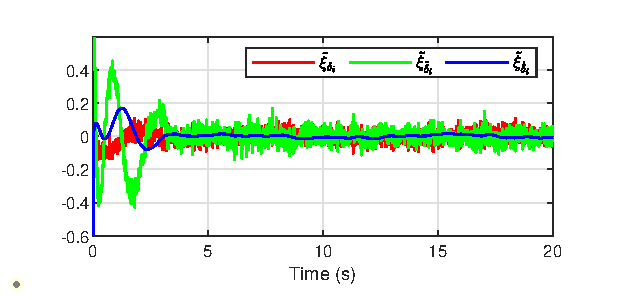
\includegraphics[scale=0.9]{ch3/img/matlab_error_case_2.eps}
    \caption{State estimation case 1.}%under the attack~\eqref{attack1}} 
    \label{fig:case1}
\end{figure}


\begin{figure}
    \centering
    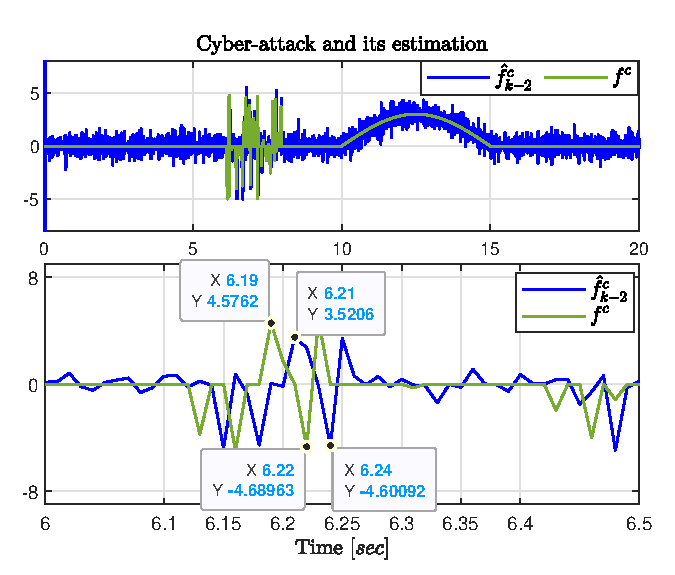
\includegraphics[scale=0.7]{ch3/img/matlab_fc_2.eps}
    \caption{Attack estimation using UIO case 1.}
    \label{fig:case1_fc}
\end{figure}


%  (since the plot of the results for this scenario
% is almost the same as Fig. 8, it is omitted to avoid repetition)
%{\color{blue}


For the second case of time-varying and bounded attack signal~\eqref{attack2}, it can be observed from the Figure~\ref{fig:case2_fc} that the cyberattack signal is accurately estimated, and the estimation error is bound.


\begin{figure}
    \centering
    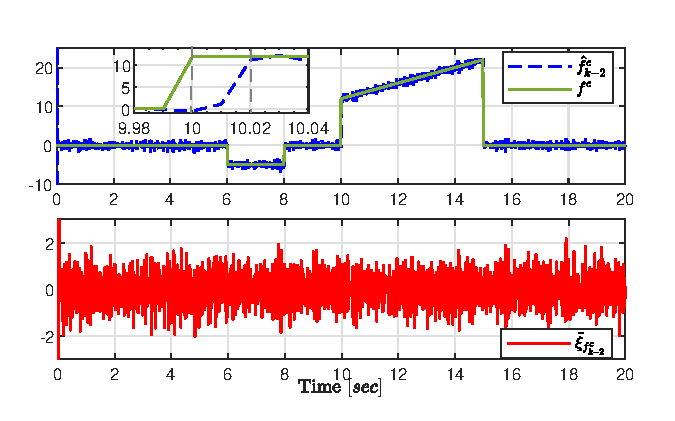
\includegraphics[scale=0.8]{ch3/img/matlab_fc_1.eps}
    \caption{Attack estimation and the errors case 2.}
    \label{fig:case2_fc}
\end{figure}

We can see that the proposed observer can estimate the the full state with good accuracy, while the unknown input is reconstructed with a fixed delay of two units based on the available output measurements. 

%}

%\begin{comment}
%
%\begin{figure}[h!]
%    \centering
%    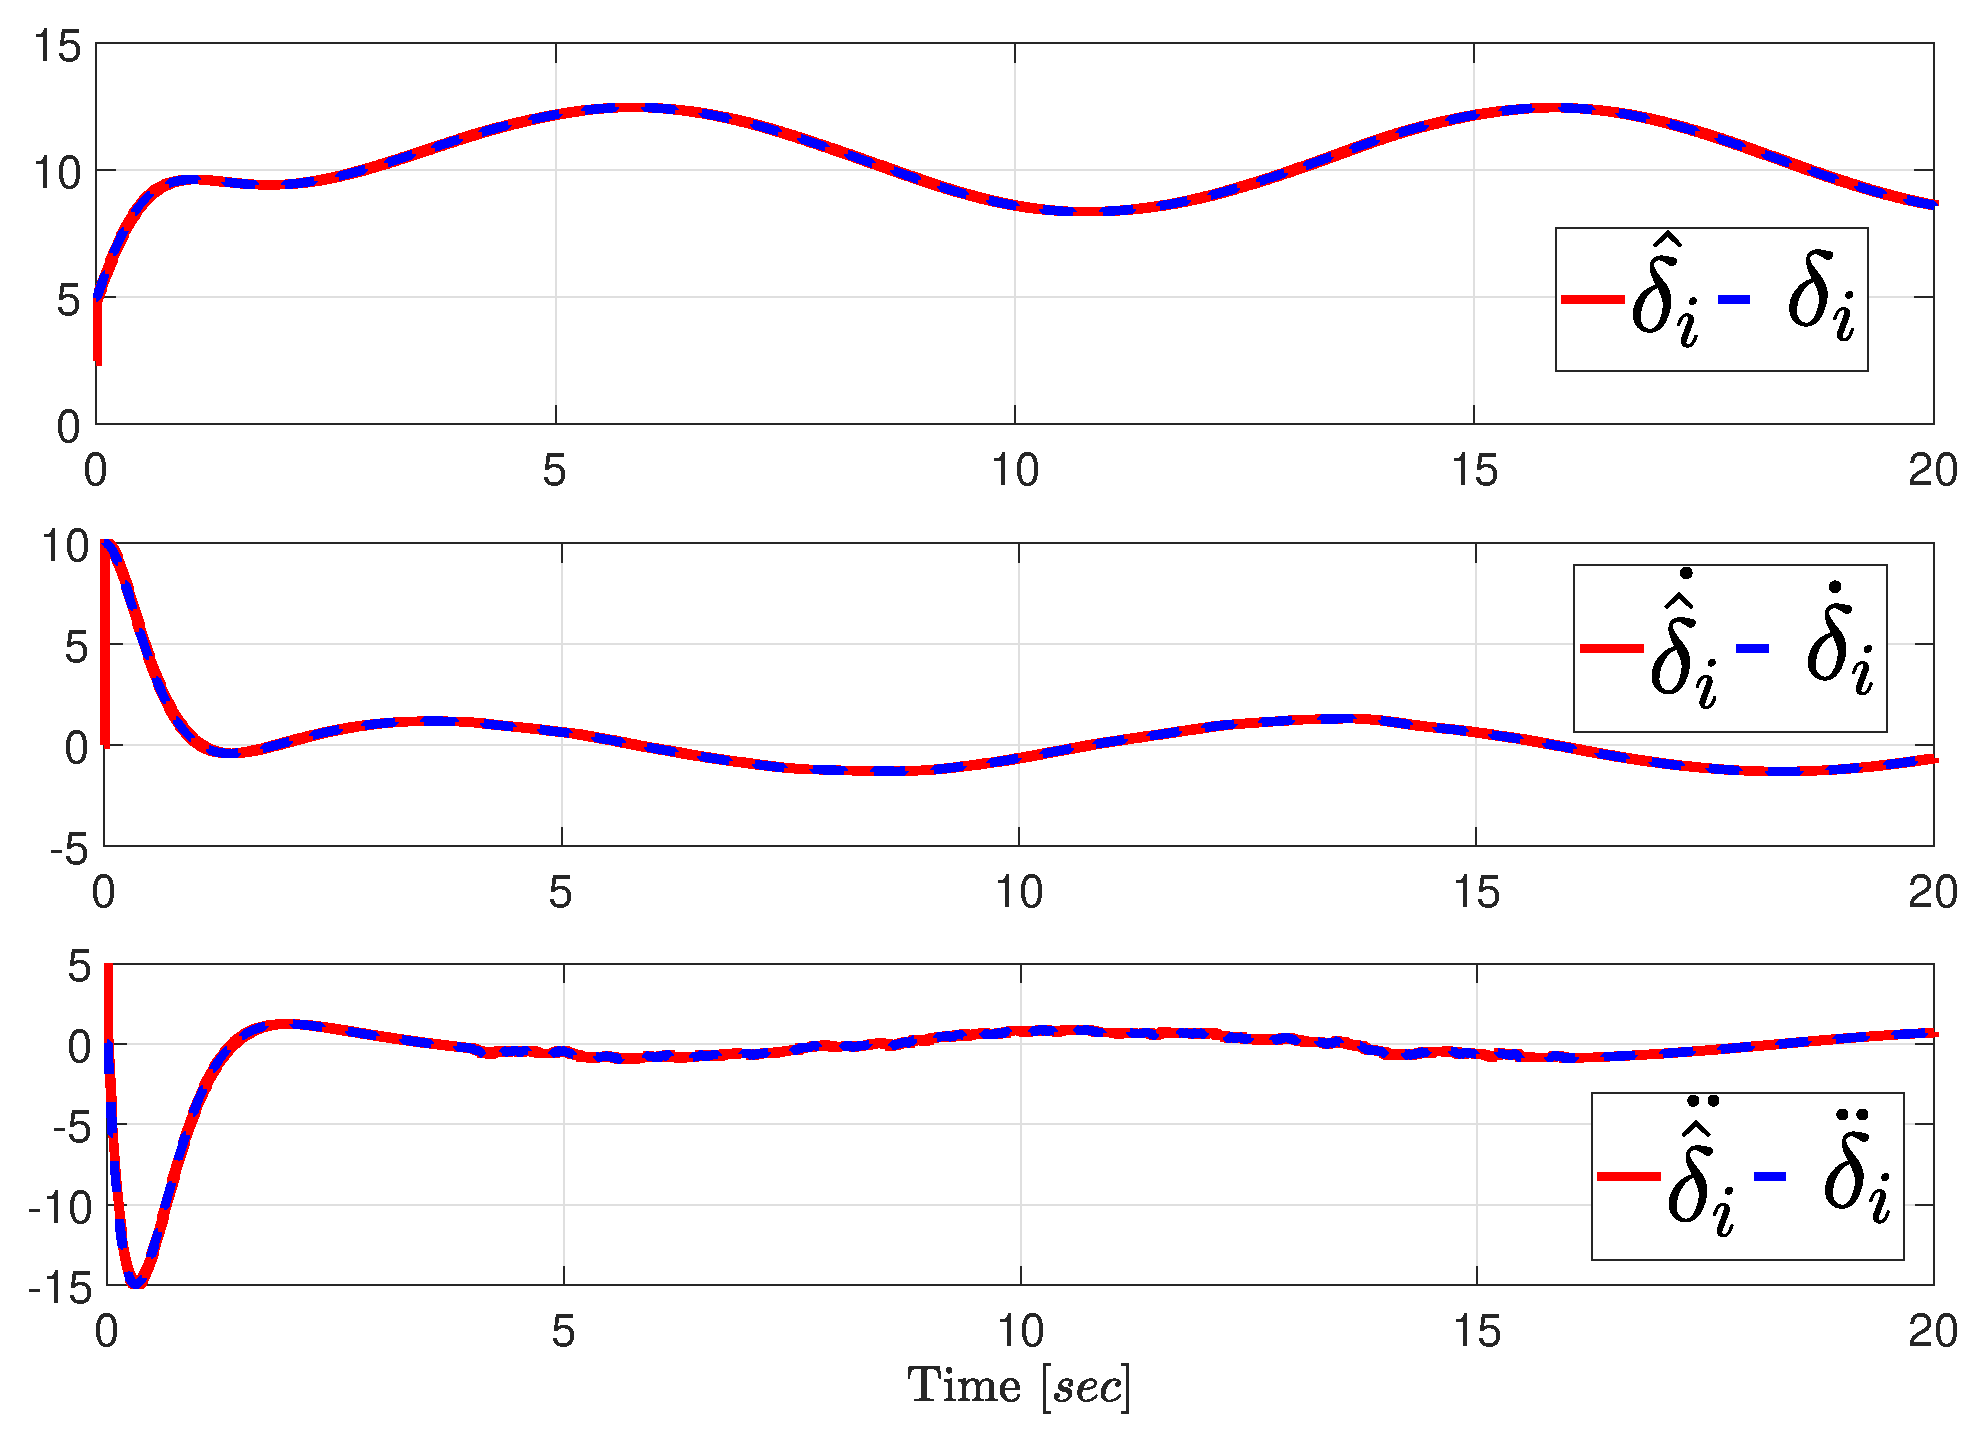
\includegraphics[width=0.4\textwidth, height=5cm]{img/case2.eps}
%    \caption{UIO state estimation case 2 }%under the attack~\eqref{attack2}}
%    \label{fig:case2}
%\end{figure}
%\begin{figure}
%    \centering
%    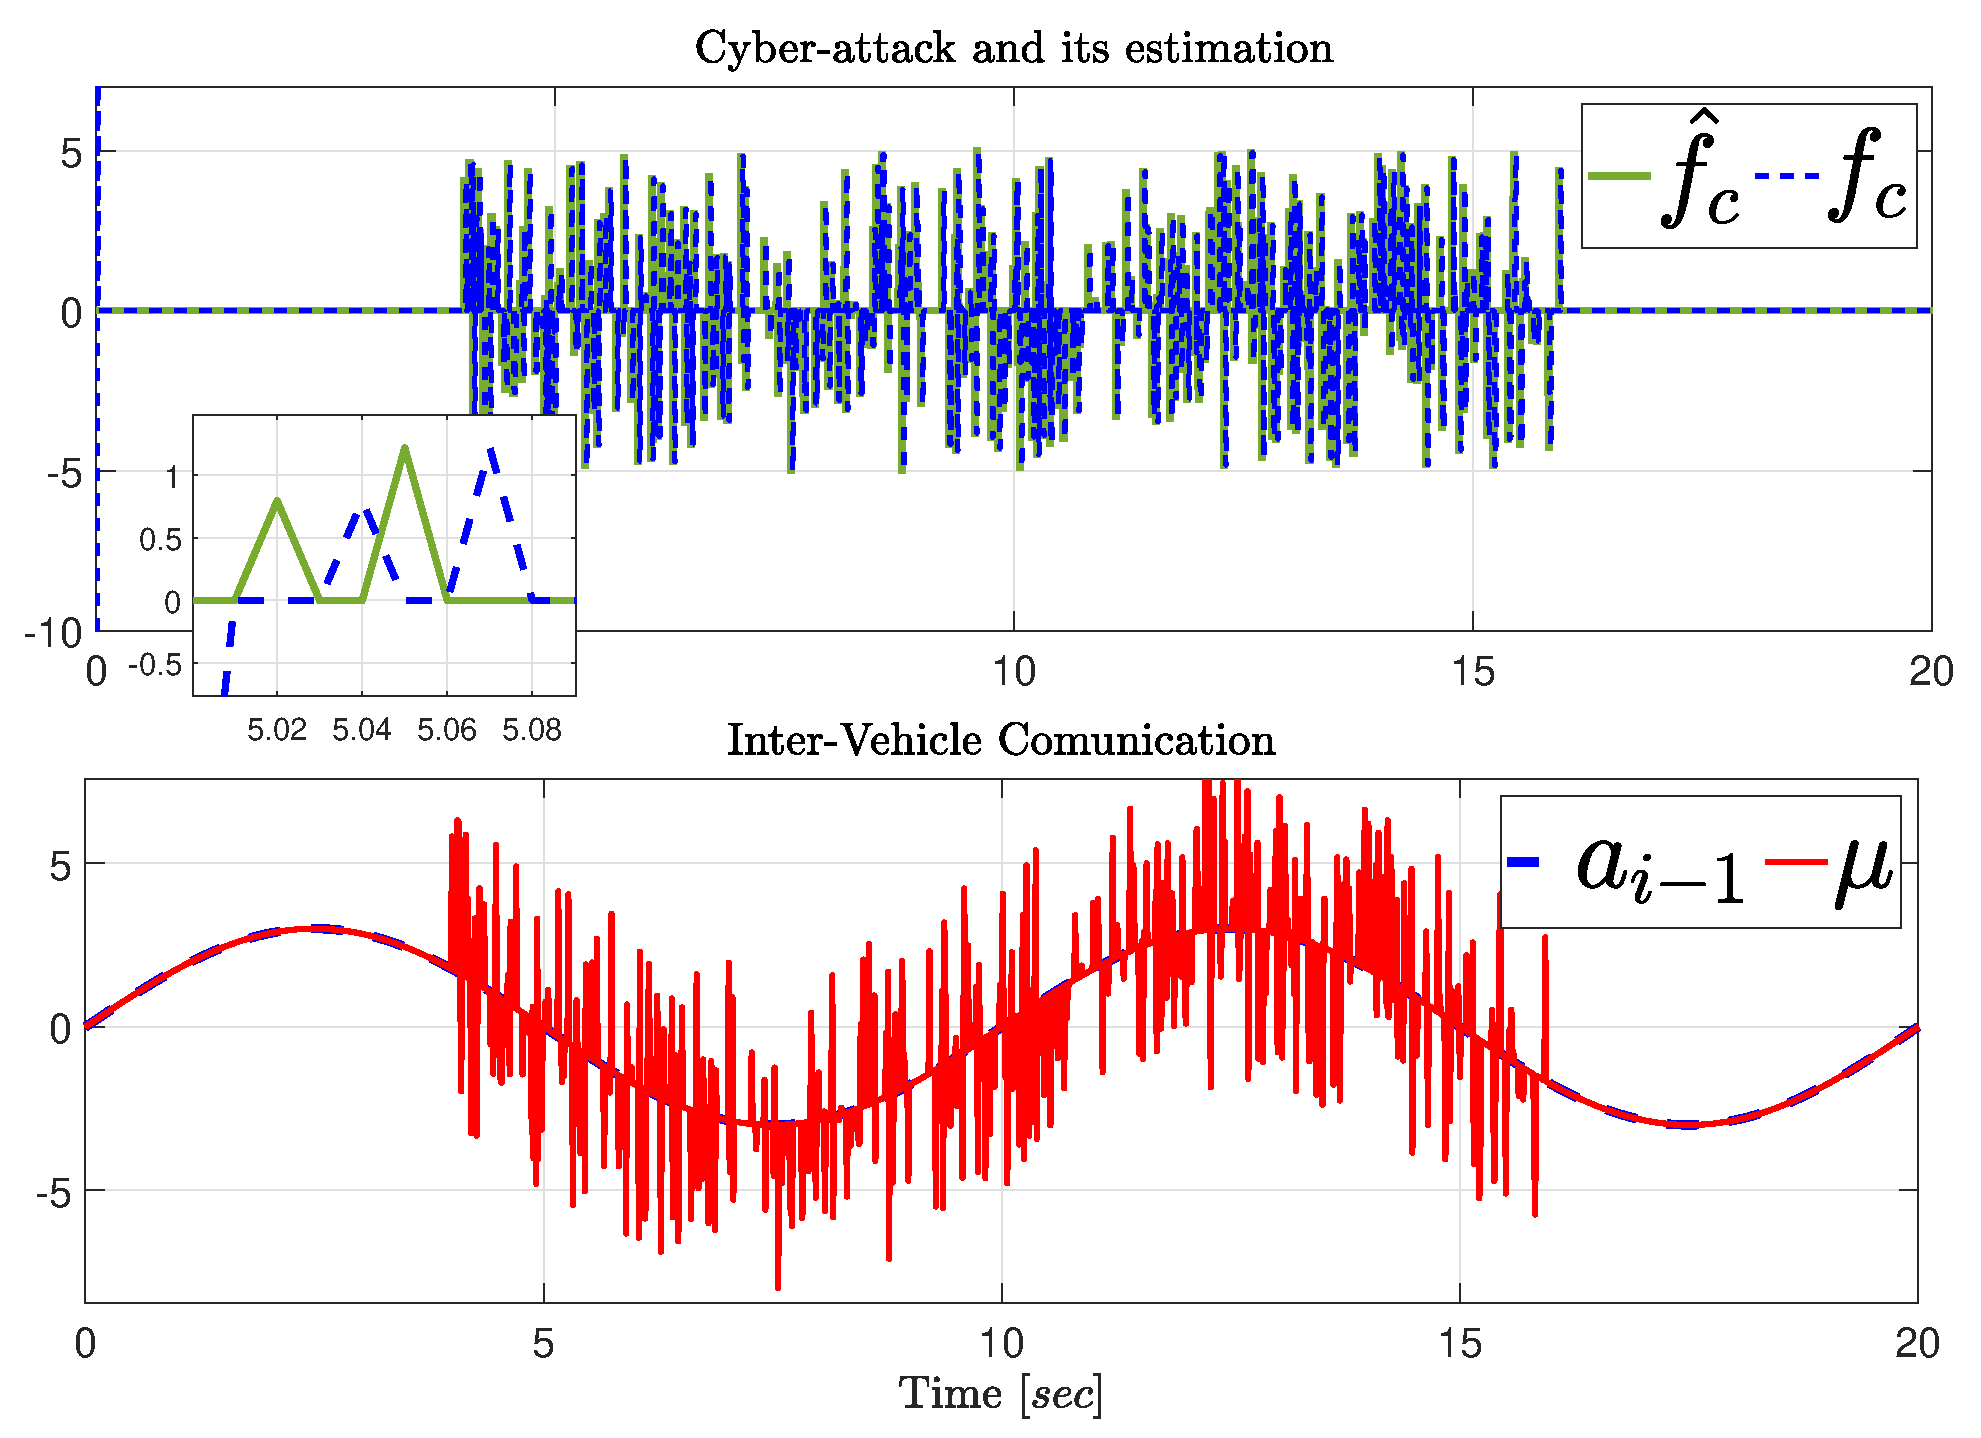
\includegraphics[width=0.4\textwidth,height = 5cm]{img/case2_fc.eps}
%    \caption{Attack estimation by UIO, case 2}
%    \label{fig:case2_fc}
%\end{figure}
%\end{comment}
%
%\begin{comment}
%    
%\pagebreak 
%\begin{remark}
%If the disturbance $\omega_{t}$ affects the second part of the state vector, $\dot{\delta}_i$, in either the system or measurement, it will impact the system's accuracy in estimating the attack $f^c$. Therefore, detecting attacks is only possible if the measurement of relative velocity remains untainted.
%\end{remark}
%
%\end{comment}

% \vspace*{-0.3cm}
\subsection{Simulation result using Carla}
%----
{
\color{black}

To evaluate the system under more realistic conditions, we conducted simulations within the CARLA simulator. Specifically, we simulated a scenario where a leading vehicle utilized a PID controller for cruise control, aiming to maintain a velocity of $10m/s$. We kept the parameters consistent with those listed in Table~\ref{tab:simple} and adopted a time step of $t_s = 0.04$. We also implemented a deterministic attack signal that varies over time and is defined by equation~\eqref{attack2}. As depicted in Fig~\ref{fig:carla_state}, the error state vectors for relative position and relative velocity exhibit good tracking, but the third vector $\tilde{\xi}_{a}$ falls short of perfection. This is because the acceleration of the preceding vehicle in Fig~\ref{fig:carla_fc} sent to the network is inconsistent, which affects the attack estimation performance. Fig~\ref{fig:carla_fc} illustrates the observer taking at least 5 seconds to converge to the actual state, and the estimated value being influenced by noise and imperfection of the model. However, the leading vehicle retains its ability to detect the cyberattack signal, ensuring a safe distance effectively}. A video showcasing the simulation scenario is provided in~\href{https://github.com/kslhuy/CACC_UIO_simulink}{GitHub repository}. Fig.~\ref{fig:carla_img} displays a thumbnail from the video.
 %~\cite{CarlaSimulator}
 \begin{figure}[h!]
     \centering    
     \includegraphics[width=0.4\textwidth,height = 3.5cm]{ch3/img/carla_d.png}
    \caption{Carla Simulator platform~(\href{https://github.com/kslhuy/CACC_UIO_simulink}{GitHub repository}).}
     \label{fig:carla_img}
 \end{figure}

\begin{figure}[h!]
    \centering    
    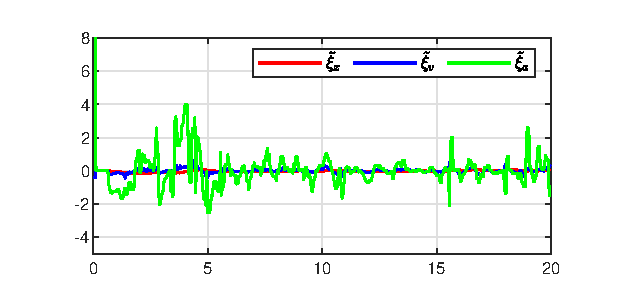
\includegraphics[scale=0.9]{ch3/img/state_carla_new.eps}
    \caption{State estimation using CARLA under attack case 2.}
    \label{fig:carla_state}
\end{figure}
\begin{figure}[h!]
    \centering    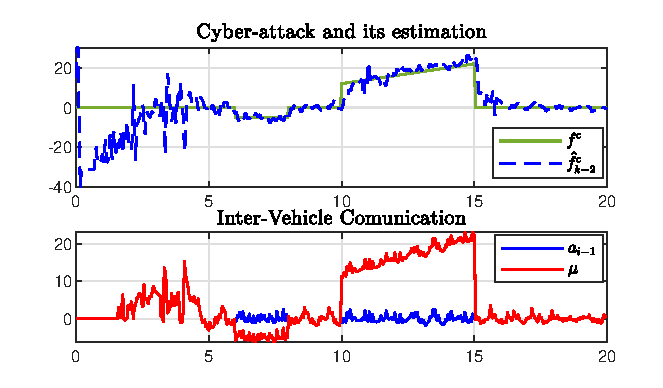
\includegraphics[scale=0.8]{ch3/img/fc_carla_new.eps}
    \caption{Cyberattack signal and inter-vehicle communication case 2.}
    \label{fig:carla_fc}
\end{figure}
%[GitHub repository](https://github.com/kslhuy/CACC_UIO_simulink).

% \pagebreak 

\section{Conclusion}
%The main contribution of this work is a new method to design a discrete-time unknown input observer in the case of unmatched faults for CACC system. The state-space representation of the system has been expressed, and the problem of false data injection via wireless communication was introduced. The derived model showed the unverified matching condition which disables unknown input observer design. To circumvent this restriction, a shift on the output of the system was applied to obtain a new system that does verify the matching condition. Afterwards, a discrete-time unknown input observer was designed and the necessary conditions for exponentially robust convergence with respect to bounded additive noise were given in terms of LMIs. Simulations confirm the effectiveness of the proposed method. The ego vehicle maintains a safe distance from the preceding vehicle, accurately reconstructs diverse-dynamic cyberattacks, and the controller is resilient against cyberattacks and bounded external disturbances.
%--

In this paper, we proposed a novel UIO design technique ensuring a theoretical ISS bound on the cyberattack detection error in the context of the CACC system. To guarantee such an ISS bound, a new LMI condition is proposed. The key idea consists in shifting the original output measurement to satisfy the well-known matching condition. The theoretical result is validated through two simulation scenarios of cyberattacks by using the Matlab software and the Carla simulator. 

Our future endeavors will focus on exploring the challenge in the presence of model parameter uncertainties. This will entail designing a robust observer-based controller, necessitating simultaneous synthesis of the observer and controller gains by addressing a unified LMI condition.











%======
\section{Exact discretization}\label{sec3}
%---

To overcome the above limitation, we propose discretizing the system. Previous studies \cite{nguyen2020cyberattack} have applied state discretization with a delay that satisfies the necessary rank condition. 
This approach represents an alternative solution to the rank condition problem. However, the introduction of delays can affect control system performance and stability, leading to reduced responsiveness and complicating the design of the observer and controller, especially in the presence of measurement noise. 
To address these challenges, we propose the use of an exact discretization method, as suggested in the literature \cite{M.Zhang} allowing us to estimate both the state and cyberattacks using an UIO. 
Additionally, we will introduce conditions to ensure the exponential convergence of the estimation error, which will be discussed in the next section.

Figure \cref{fig_dis_UIO} illustrates the structure of the proposed observer-based cyberattack estimation framework.

\begin{figure}[h!]
\centering
\includegraphics[width=7cm]{ch3/img/probleme_2.png}
\caption{Discrete-time model-based UIO}
\label{fig_dis_UIO}
\end{figure}



The discrete-time version of equation is presented as follows, according to the approach detailed in reference \cite{M.Zhang}:




\begin{equation}\label{CACC_discrete}
%\displaystyle
      \left\{ \begin{array}{l}
        x_{k+1} = A_d x_{k} + B_d v_{i,k} +F_d  \mu_{k}+ \hat{\Delta} - W_d  f^c_{k} \\
            y_{k} = C_d x_{k}\end{array}\right.
\end{equation}  
where 
\begin{align*}
    A_d = e^{A_c T_s},\, B_d =\,\int_{0}^{T_s} e^{A_c \eta} B_c d\eta, \, C_d = C_c
\end{align*}

$$F_d = \int_{0}^{T_s} e^{A_c \eta} F_c d\eta,\, W_d = \int_{0}^{T_s} e^{A_c \eta} W_c d\eta,\,  
$$ 
\begin{align*}
\hat{\Delta} = \int_{0}^{T_s} e^{A_c \eta} \Delta \eta
\end{align*}

and $T_s$ is a sampling period

We verify the rank condition of the newly discretized system (6) :

\[
C_d W_d = \begin{pmatrix}
1 & 0 & 0 \\
0 & 1 & 0
\end{pmatrix} 
\begin{pmatrix}
1.14e^{-06}\\
      3.41e^{-04}\\
      6.75e^{-02}
\end{pmatrix} 
= 1e^{-03}\begin{pmatrix}
    0.0011\\
    0.3419
\end{pmatrix}
\]

The rank condition is satisfied:
\[
\text{rank}(CW) = \text{rank}(W)
\]


